Lo primero que se realiz\'o fue una optimizaci\'on de la energ\'ia de corte y a 
continuaci\'on una optimizaci\'on de las dimensiones de la grilla de puntos k 
en la red reciproca con el fin de 
mejorar la precisi\'on de los resultados que se obtendr\'an al estudiar las 
propiedades de los materiales.

\subsection{Energ\'ia de corte}

La energ\'ia de corte es un par\'ametro importante, ya que define la 
cantidad de ondas planas consideradas para expandir las funciones de 
onda. Este par\'ametro es dependiente del sistema, es decir, que debe 
calcularse para ajustarse a los \'atomos que componen el sistema y al 
pseudopotencial utilizado. Para determinar el valor \'optimo del par\'ametro 
para 
ambos materiales, se realizaron varias simulaciones probando distintos valores 
en un intervalo de 20 Ry hasta 100 Ry con una variaci\'on de 5 Ry entre cada 
valor, siendo un total de 17 valores distintos. La energ\'ia de corte se 
determin\'o como el menor valor a partir del cual la energ\'ia total no varia 
considerablemente. 

\noindent Para el $BiFeO_{3}$ se obtuvo que la energ\'ia de corte optima es 40 
Ry, como 
se puede observar en la gr\'afica \ref{energia_corte_BFO}

\begin{figure}[H]
    \centering
    \includegraphics[width=0.7\textwidth]{contenido/resultados/optimizacion/img_optimizacion/energia_corte_BFO.png}
    \caption[Energ\'ia de corte $BiFeO_{3}$]{Energ\'ia de corte optima 
        para el $BiFeO_{3}$}
    \label{energia_corte_BFO}
\end{figure}

\noindent Para el $YCrO_{3}$ se obtuvo que la energ\'ia de corte optima es 40 
Ry, como 
se puede observar en la gr\'afica \ref{energia_corte_YCO}

\begin{figure}[H]
    \centering
    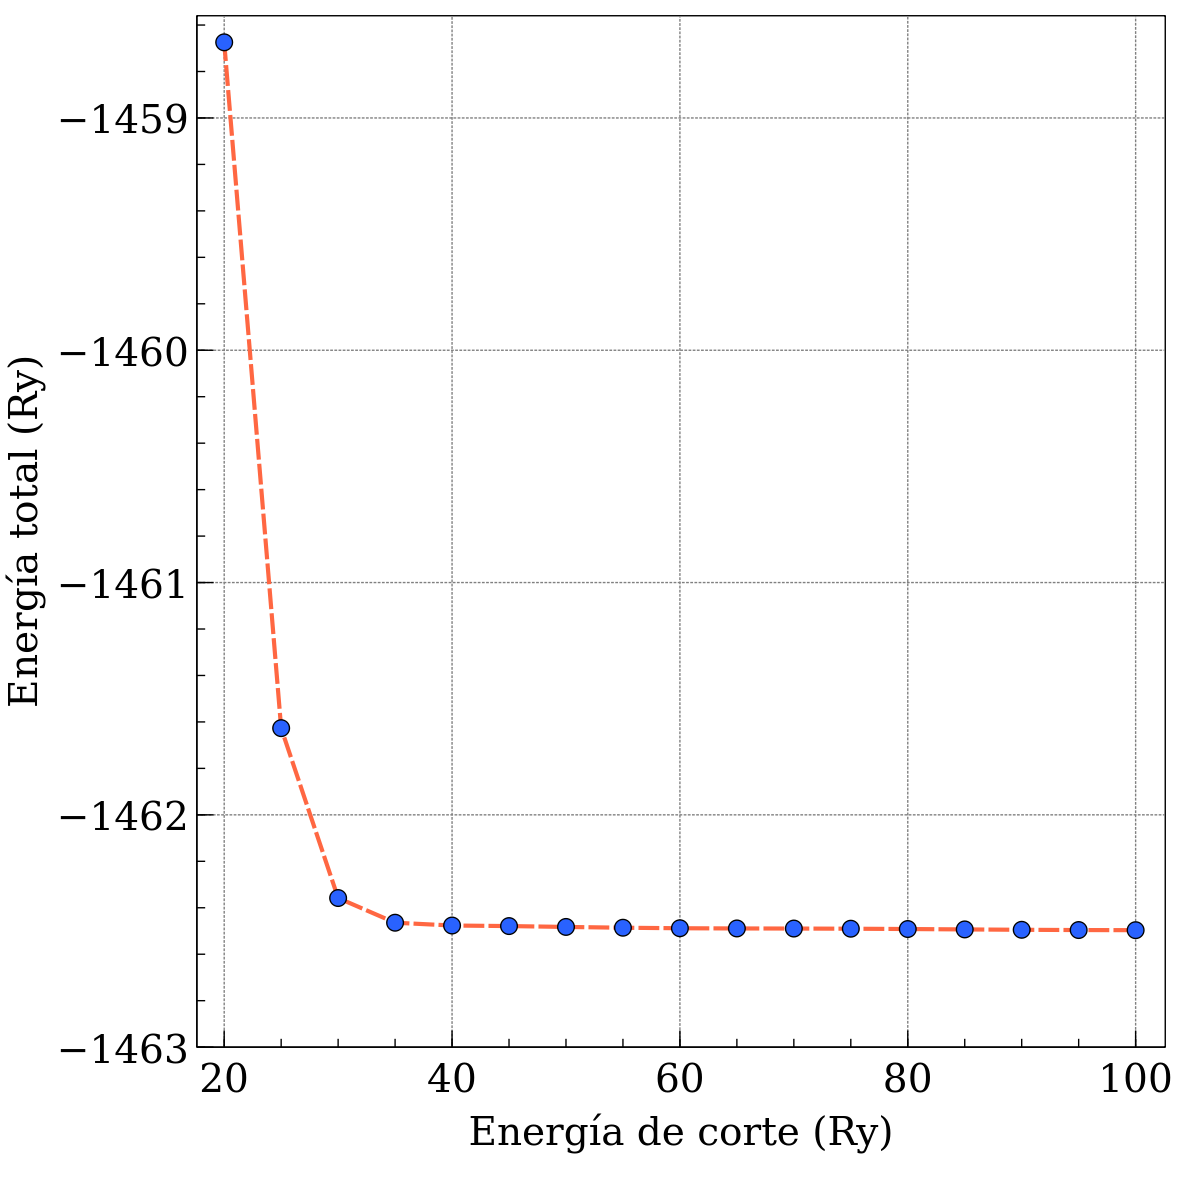
\includegraphics[width=0.7\textwidth]{contenido/resultados/optimizacion/img_optimizacion/energia_corte_YCO.png}
    \caption[Energ\'ia de corte $YCrO_{3}$]{Energ\'ia de corte optima 
        para el $YCrO_{3}$}
    \label{energia_corte_YCO}
\end{figure}

\noindent Como se mencion\'o la energ\'ia de corte es un par\'ametro 
importante. Esto es 
debido a que el conjunto de ondas planas es infinito lo cual es un problema 
para llevar a cabo una simulaci\'on. Este problema se soluciona imponiendo un 
limite en el n\'umero de ondas planas utilizadas, dicho limite es la energ\'ia 
de corte. Es posible considerar ondas planas m\'as all\'a de la energ\'ia de 
corte pero el aumento en la precisi\'on de los resultados es muy peque\~no y no 
justifica el aumento del tiempo de simulaci\'on y de la capacidad de c\'alculo 
computacional requerida para concretar la simulaci\'on.

\subsection{Dimensi\'on de la grilla de puntos K}

Muchas cantidades que necesitamos evaluar involucran integrales sobre la 
primera zona de Brillouin. En la pr\'actica, las integrales se discretizan 
asociando un peso a los puntos K que se consideran.
La dimensi\'on de la grilla de puntos K en la red reciproca debe optimizarse 
con el fin de mejorar la precisi\'on de los 
c\'alculos y reducir el tiempo de simulaci\'on. Para determinar las dimensiones 
\'optimas de la grilla de puntos K para ambos materiales, se realizaron varias 
simulaciones probando varios tama\~nos de grilla. El paquete Quantum Espresso 
implementa el m\'etodo de Monkhorst-Pack para el cual se deben indicar tres 
valores correspondientes a los tres ejes espaciales. Para el $BiFeO_{3}$ se 
utilizaron grillas en el intervalo de $2 \times 2 \times 2$ hasta $9 \times 9 
\times 9$ y para el $YCrO_{3}$ se utilizaron grillas en el rango de $2 \times 2 
\times 2$ hasta $10 \times 10 \times 10$.

\noindent Para el $BiFeO_{3}$ se obtuvo que la grilla optima es de $6 \times 6 
\times 6$, 
como se puede observar en la gr\'afica \ref{puntos_k_BFO}.

\begin{figure}[H]
    \centering
    \includegraphics[width=0.7\textwidth]{contenido/resultados/optimizacion/img_optimizacion/energia_kp_BFO.png}
    \caption[Dimensi\'on de la grilla de puntos k $BiFeO_{3}$]{Dimensi\'on de 
    la grilla de puntos k \'optima para el $BiFeO_{3}$. El eje inferior muestra 
    solo el valor en una dimensi\'on por claridad, dado que la definici\'on 
    real es en tres dimensiones $a \times a \times a$}
    \label{puntos_k_BFO}
\end{figure}

\noindent Para el $YCrO_{3}$ se obtuvo que la grilla \'optima es de $6 \times 6 
\times 6$, 
como se puede observar en la gr\'afica \ref{puntos_k_YCO}.

\begin{figure}[H]
    \centering
    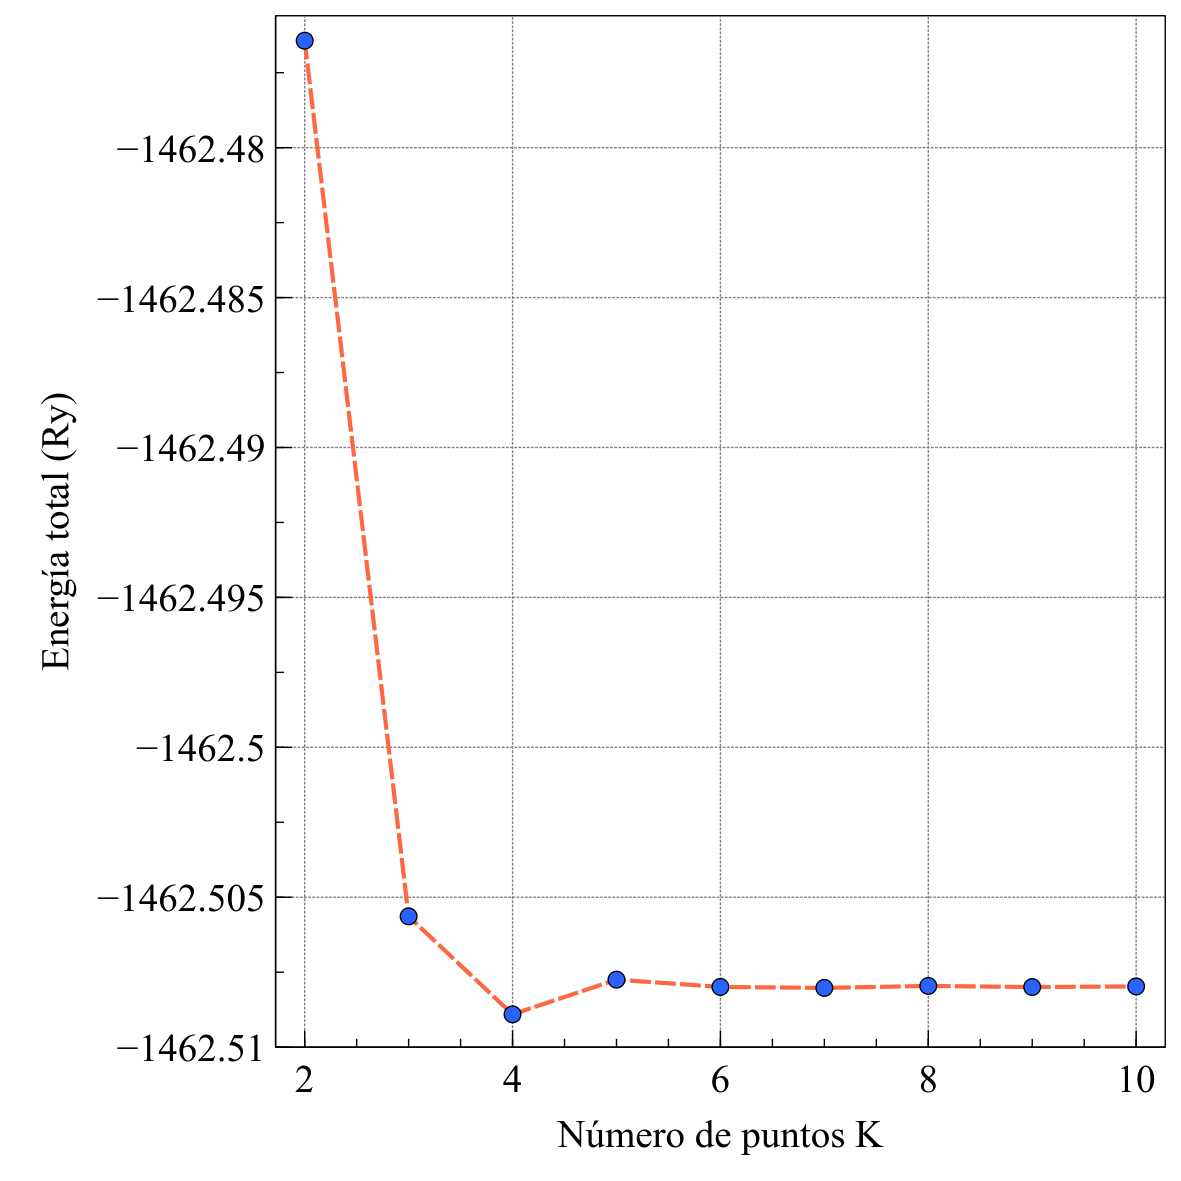
\includegraphics[width=0.7\textwidth]{contenido/resultados/optimizacion/img_optimizacion/energia_kp_YCO.png}
    \caption[Dimensi\'on de la grilla de puntos k $YCrO_{3}$]{Dimensi\'on de 
        la grilla de puntos k \'optima para el $YCrO_{3}$. El eje inferior 
        muestra solo el valor en una dimensi\'on por claridad, dado que la 
        definici\'on real es en tres dimensiones $a \times a \times a$}
    \label{puntos_k_YCO}
\end{figure}
